\documentclass{bioinfo}
\usepackage[english]{babel}
\copyrightyear{2015} \pubyear{2015}
\usepackage{natbib}
\bibliographystyle{natbib.bst}


\access{Advance Access Publication Date: Day Month Year}
\appnotes{Manuscript Category}

\renewcommand{\cite}{\citep}
\usepackage{todonotes}

\begin{document}
\firstpage{1}

\subtitle{Subject Section}

\title[short Title]{Combining Bottom-up and top-down approaches through graph learning over interaction networks for drug-target-interaction prediction}
\author[Sample \textit{et~al}.]{Tilman Hinnerichs\,$^{\text{\sfb 1,}*}$ and Robert Hoehndorf\,$^{\text{\sfb 2}}$}
\address{$^{\text{\sf 1}}$Department, Institution, City, Post Code, Country and \\
$^{\text{\sf 2}}$Department, Institution, City, Post Code,
Country.}

\corresp{$^\ast$To whom correspondence should be addressed.}

\history{Received on XXXXX; revised on XXXXX; accepted on XXXXX}

\editor{Associate Editor: XXXXXXX}

\abstract{\textbf{Motivation:} Text Text Text Text Text Text Text Text Text Text Text Text Text
Text Text Text Text Text Text Text Text Text Text Text Text Text Text Text Text Text Text Text
Text Text Text Text Text Text Text Text Text Text Text Text Text Text Text Text Text Text Text
Text Text Text Text Text Text
Text Text Text Text Text.\\
\textbf{Results:} Text  Text Text Text Text Text Text Text Text Text  Text Text Text Text Text
Text Text Text Text Text Text Text Text Text Text Text Text Text  Text Text Text Text Text Text\\
\textbf{Availability:} Text  Text Text Text Text Text Text Text Text Text  Text Text Text Text
Text Text Text Text Text Text Text Text Text Text Text Text Text Text  Text\\
\textbf{Contact:} \href{tilman.hinnerichs@kaust.edu.sa}{tilman.hinnerichs@kaust.edu.sa}\\
\textbf{Supplementary information:}10264703 Supplementary data are available at \textit{Bioinformatics}
online.}

\maketitle
\section{Introduction}

\cite{Survey2018}\\
In history, traditional remedies, that were known for their medicinal
properties lead to drugs by extraction of the functional
ingredients. Alternatively, characteristics and features of potential
drugs were detected by accident like in the case of penicillin. More
recently, biological drug targets can be found \textit{in silico}
through discovery of suitable computational predictors.


The challenge of accurately predicting drug-target-interactions (DTI)
has shown its importance in the fields of drug repurposing and
repositioning, and in the exploration of novel drugs and their
interaction partners. Knowledge about those links between compounds
and their target proteins help in an array of medical and
pharmaceutical studies. Additionally, those associations can be
utilized to identify disease specific targets, leading to desirable
therapeutic effects.

With the rapidly growing field of machine learning approaches and
their application to bioscientifical problems in the realm of
bioinformatics, different kinds of data, such as long DNA sequences
could be utilized for feature generation, while rapid advances were
made. Almost all state of the art models for drug-target-interaction
prediction were based on the usage of neural networks with increasing
size.\todo{Needs ref, or reformulate}

Only recently, the technique of graph learning was introduced by
\citet{GCNConv} through graph convolution algorithms, and improved and
altered under usage of different kernels \cite{ChebConv, ARMAConv},
attention mechanisms \cite{GATConv}, random walks \cite{APPNPConv},
and mixtures of both \cite{SAGEConv}. While based on diverse systems,
they can be relevant for testing distinct hypothesis for given
graphs. While convolutional filters are suitable for finding patterns
among the the given graph, attention mechanisms are more relevant for
discovery of important regions within. Lately, graph learning
approaches found application for computing compound representations
for DTI prediction.

Approaches on this rather sophisticated\todo{Try to avoid}
problem\todo{Need to state the problem clearly here or at end of prev
  paragraph} can divided into top-down or network approaches
(\textbf{CITATION}), and bottom-up or molecular approaches
(\textbf{CITATION}). Top-down approaches take advantage of other data
such as diseases (CITATION), side effects, knowledge graphs or
ontologies, in order to learn representations for both compound and
protein. \todo[inline]{We call these approaches ``top-down'' because
  they start with the observable characteristics induced by a drug and
  infer the targets based on the likely molecular mechanisms that
  result in these phenotypes.} On the other hand, bottom-up approaches
attempt to learn from chemical properties of proteins or drugs to
infer candidate drug--target interactions. For drugs, molecular
structure (CITATION GraphDTA), molecular fingerprints, similarity to
other drugs (See Bioinf Survey), and other molecular features may be
used. On the protein side, secondary structure prediction (CITATION),
contact prediction (CITATION), or simply\todo{Don't use ``simply''.}
convolution over the amino acid sequences can be used to obtain a
feature representation for a given proteins. However, both bottom-up
and top-down approaches to drug--target interaction prediction
\todo[inline]{replace: ``contain and share some problems'' with
  something like ``have some limitations''} that are not solvable within
themselves.
\todo[inline]{Following is not sufficiently precise; here, you need to
clearly state the challenges faced by both approaches, ideally with
references.}
Thus, bottom-up approaches share the lack of ability to
generalize, which we will show in later sections, and usually focus on
engineering sophisticated features for the drugs, while neglecting to
formulate meaningful features on the protein side. Top-down approaches
lack the ability to spot small differences to cope with small
differences within the drug structure and rely heavily on given data
for the considered drug-target pair. The latter is not suitable for
predictions on novel or unseen compounds, as e.g., data on side
effects or its impact on diseases is seldom given for novel drugs.

In order to design such a feature for proteins and drugs,
respectively, we make use of the interaction networks for both
proteins and compounds. Drug-drug interaction networks were introduced
and standardized by \citet{Boyce2015} and have been used for clinical
decision support \cite{Scheife2015}. Drug-drug interaction networks
may give a hint on common targeted pathways. As an additional compound
feature we will use semantic side effect similarity, which we will
discuss later on\todo{Generally, try to avoid pointers to ``later''.}.

Protein-protein interaction networks have shown great results in $\dots$(\cite{Vazquez2003}, \cite{Ackerman2019}) in granting context for molecular system biology. However, these contexts were never applied to the problem of drug-target-interaction prediction. Thus we formalized our hypotheses over these interaction graphs and will test them in the following chapters.

\enlargethispage{12pt}

\section{Methods}
\subsection{Datasets}
The data for the different parts of this model were obtained from various sources. Starting with the protein-protein interactions, we fetched 11.574 proteins with over 170.000 links from STRING (\cite{STRINGv10}). For the drug-target interactions themselves, we fetched 
137.000 links from STITCH database (\cite{STITCHv5}). As both STRING and STITCH provide probability scores for each association, we filtered them as advised by a threshold of 700, thus only obtaining likely interactions.\\
For the ontology segment we utilized PhenomeNET \citep{PhenomeNET2011}, a collection of various ontologies such as Human Phenotype Ontology \citep{HPO2018}, Gene Ontology (\citet{GOoriginal2000} \citet{GOrecent2020}), Mammalian Phenotype Ontology \citep{MP2009} and numerous others. \todo{which ontologies to cite}
Side effects and their links to drugs were obtained Side Effect Resource (SIDER)\citep{SIDER} and structured according MedDRA database \citep{MedDRA}. They were mapped to PhenomeNET with aid of \textit{Phenomebrowser.net}, which provides a SPARQL query endpoint for the mentioned resources. \\

We additionally obtained molecular structure based features for drugs from \textit{SmilesTransformer}\citep{SmilesTransformer} and proteins from \textit{DeepGOPlus}\citep{DeepGoPlus}.\\
 
Eventually the intersection between these resources yielded \todo{num drugs} drugs and \todo{num proteins} human proteins for the training phase. We provide links to and methods for the necessary data in the provided Github repository.\\

\subsection{Problem Description}
The issue of predicting drug-target interactions can be described quite briefly: For a given drug and a given protein we want to forecast whether those interact or not. We hereby do not differentiate between activation and inhibition, and do not erect statements on the strength of the bond.\\

\subsection{Model} 
In order to build a method that incorporates both top-down and bottom-up features, we first created a model for each. In the top-down section, we used \textit{DL2vec}\citep{DL2vec2020} to obtain ontology based representations. Hereby, DL2vec constructs a graph by introducing vertices and edges for each ontology class and axiom, respectively, followed by random walks starting from each entity. These walks are eventually learned on using a Word2vec \citep{Word2vec2013} model. Thus, we pick up rich, neighbourhood focused representations for each entity, which has shown great results for representing protein function and phenotypes. \\

As we want to learn from the similarity of drug side effects and protein phenotypes we opted for a deep siamese network approach, hence learning a high-dimensional embedding emphasizing this identity by forcing a maximal cosine similarity between these embeddings. On the other hand we build a deep neural network for the molecular structure based features. \\

\subsubsection{Graph convolutional layers}
These molecular and ontology based sub-models were added to a larger graph convolutional model.
As described before, graph convolution has shown significant performance increase in a variety of tasks. While there are various methods out there we will only introduce the mose basic one here. A graph convolutional layer w.r.t. \citet{GCNConv} hereby consists of a learnable weight matrix followed by an aggregation step, formalized by

\begin{equation}
	\mathbf{X}^{\prime} = \mathbf{\hat{D}}^{-1/2} \mathbf{\hat{A}}
	\mathbf{\hat{D}}^{-1/2} \mathbf{X} \mathbf{\Theta}
\end{equation}

where for a given graph $G=(V,E)$, $\hat{A} = A + I$ denotes the adjacency matrix with added self-loops for each vertex, $D$ is described by $\hat{D}_{ii} = \sum_{j=0} \hat{A}_{ij}$, a diagonal matrix displaying the degree of each node, and $\Theta$ denotes the learnable weight matrix. Added self-loops enforce that each node representation is directly dependent on its own preceding one. Notably, the number of graph convolutional layers stacked equals the radius of relevant nodes for each vertex within the graph.\\

The update rule for each individual node is denoted by 

\begin{equation}
	\mathbf{x}^{\prime}_i = \mathbf{\Theta} \sum^{N}_{j}
	\frac{1}{\sqrt{\hat{d}_j \hat{d}_i}} \mathbf{x}_j
\end{equation}

where both $\hat{d}_i, \hat{d}_j$ are dependent on the edge weights $e_{ij}$ of the graph. With simple, single valued edge weights such as $e_{ij}=1 \text{ }\forall (i,j)\in E$, all $\hat{d}_i$ reduce to $d_i$, i.e. the degree of each vertex $i$. \\

While in this initial formulation the node-wise update step is defined by the sum over all neighbouring node representations, we are able to alter this formulation for a more sophisticated message passing scheme. As described we are able to rearrange the order of activation function, aggregation and linear neural layer with this formulation as proposed by \citet{GENConv2020}:

\begin{equation}
	\mathbf{x}_i^{\prime} = \mathrm{MLP} \left( \mathbf{x}_i +
	\mathrm{AGG} \left( \left\{
	\mathrm{ReLU} \left( \mathbf{x}_j + \mathbf{e_{ji}} \right) +\epsilon
	: j \in \mathcal{N}(i) \right\} \right)
	\right)
\end{equation}

While the reordering is merely import for numerical stability, the authors claim that this alteration of the original formulation eases the vanishing gradient problem for deeper convolutional networks. \\




\subsection{Choosing a train-test splitting scheme}
In general, drug-target interaction prediction is the task of accurately predicting, whether for a given drug and a given protein there is a biological interaction within the target organism. Hereby, different training and prediction schemes lead to divergent expressiveness of the resulting model. However, when building the train-test split over compound-protein pairs for building the actual model, there are the following three options:

\begin{enumerate}
	\item Build split over drugs
	\item Build split over drug-target pairs
	\item Build split over proteins
\end{enumerate} 
In general, recent works do perform their split over the drugs or drug-target pairs (\cite{Survey2018}, CITATION). As there are hopefully many more drugs to discover, the drug split scheme both emphasizes the drug repurposing idea, by applying unseen compounds to existing targets, but also benefits from more complicated drug representations, leading to tremendous results. This performance gain is based on minor variations among large groups of pharmaceuticals, that are easy to acquire. The second scheme has knowledge on all drugs and all proteins, and is thus prone to overfitting and the same development bias. Eventually, as there only limited drug-targets \citep{Overington2006}, predicting per protein is rather counter-intuitive. As it is hard to generalize over proteins representations, we aim at reaching similar performances for both drug and protein splitting schemes. \\

In general, recent works do perform their split over the drugs or drug-target pairs (\cite{Survey2018}, CITATION). The first is more relevant for novel drugs, as it is much more likely to test a new compound than a innovative protein. However, it lies in the very nature of the used datasets, making the prediction for new drugs much easier. Thus, drugs are often built by minor variations of existing drugs, thus leading to no deviations in the functional group of that very compound (CITATION/EXAMPLE). When distributed over both train and test split, the models do not perform inductive inference and generalize, but rather implement transductive inference by just predicting the recently seen structures. Hence, when entirely new molecules are seen, the models perform much worse. \\
The same applies to splits of drug-target pairs, as all drugs were already seen, and novelty cannot be coped with.\\
As mentioned in the introduction it is quite difficult to learn suitable features from proteins. In general, attempts search for motifs in the protein sequences under usage of convolutional neural networks and filters, which is more suitable for tasks like protein function prediction, than for for drug-target interaction prediction, and lack a more in-depth hypothesis on the protein side, while investing in refined drug features. \\
Thus, building splitting over proteins is the most challenging of the three options. \\

\subsection{Tested hypotheses}

In this work we are testing the following hypotheses:
\begin{enumerate}
	\item Can we build a model that outperforms state of the art approaches, combining top-down and bottom-up approaches?
	\item Are interaction networks sufficient to improve the performance of simple molecular predictors?
\end{enumerate}
We will test the first hypothesis by building a model that takes both top-down and bottom-up features into account. Thus, we propose a novel approach to combine those mutual exclusive attempts, through the usage of interaction networks, similarity and molecular features. Additionally, we test the latter by building a simple molecular DTI predictor and enhance it under usage of the interaction networks.\\

For the bottom-up approach we build a model that only relies on molecular features, which we will discuss in more detail in the following methods chapter. For the combination of both approaches we now attach the predictions to the protein-protein interaction graph as node features for future graph learning steps. In this graph we tried to find both patterns and regions for each drug that could be of interest through application of different graph convolutional layers, which in return represent the feature for each protein. Representing the drug we take the drug-drug interaction graph and the semantic similarity over side effects which we will explain in the following paragraphs.

\section{Methods}

\subsection{Models}
The used model consists of two separate models, that help to fuse together the two methods:
\begin{enumerate}
	\item The molecular predictor
	\item The interaction network based predictor
\end{enumerate}
We build the molecular predictor by using pretrained, molecular fingerprints models for both drugs and proteins. Regarding proteins, we used the pretrained feature generator from \textit{DeepGoPlus} (\citep{DeepGoPlus}) that was originally designed for protein function prediction and is regarded as state of the art for this purpose. For drugs we used a pretrained fingerprint model from \textit{SMILES transformer} (\cite{SmilesTransformer}), that provides a simple and fast method to compute fingerprints through autoencoder models. The encodings from these two models were funneled into a simple deep neural network (see Figure~\ref{fig:01}) with few fully connected. \\
The results of that prediction flow into the annotation of the protein-protein interaction (PPI) graph as depicted in (IMAGE). Hereby, the predictions of the molecular predictor are used as node features for the graph, with respect to the given drug. Thus, given a compound-target pair, the nodes of the PPI graph now hold bottom-up features, which can now be processed by the graph learning algorithms. \\
The PPI graph is processed by different graph convolutional layers, that may underline the importance of either patterns or regions within the graph, to obtain a feature vector for the wanted node. In contrast to learning over whole graphs we perform node classification within the graph. These layers are either graph convolutional layers, that learn a certain kernel over the graph, or attention based. Different layers of both and other types such as were tested.  \\
The drug-drug interaction features are retrieved by choosing the corresponding row in the adjacency matrix of the graph, thus leading to quite simple features. \\
For the semantic similarity feature, that once again represents a top-down attribute, we artificially link each drug to its corresponding side effects in the MedDRA hierarchy. Concerning this hierarchy, drug-drug similarity is computed by the Resnik similarity (\cite{Resnik1995}). For the given compound we take the corresponding row of this symmetric similarity matrix. \\

Thereby, we concatenate these three features together and funnel them into another deep neural network as depicted in figure \ref{fig:02}. This network finally yields our prediction. We hereby perform splits over both drugs and proteins, in order to test and show the discrepancy and increasing difficulty.\\ Implementation was done in PyTorch (\cite{Pytorch}) and is available on Github under \href{github.com/thinnerichs/KAUST-dti-metabol}{github.com/thinnerichs/KAUST-dti-metabol}. Graph learning methods were build with help of PyTorch-Geometric (\cite{PytorchGeometric}), a geometric deep learning extension library for PyTorch, that recently got a lot of attention in the machine learning community. This library gives the potential to use many state of the art graph learning mechanisms, such as plain but effective graph convolution (\citet{GCNConv}), Chebychev kernels (\cite{ChebConv}), ARMA kernels (\cite{ARMAConv}), translation-invariant operators (\cite{FeaStConv}), attention mechanisms (\cite{GATConv}), random walks (\cite{APPNPConv}) and mixtures of the latter two (\cite{SAGEConv}). The performance of these various layer types were tested for this particular problem, as discussed in the results section.

\begin{figure}[!tpb]%figure1
	\centerline{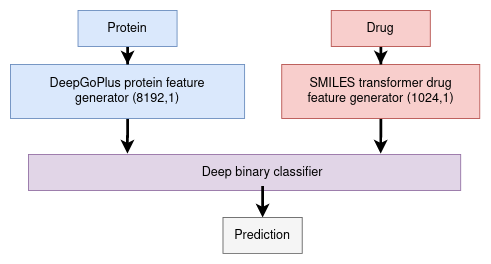
\includegraphics[width=0.4\textwidth]{figures/MolecularPredictor.png}}
	\caption{Molecular predictor based on the generated features from DeepGoPlus and SMILES transformer.}\label{fig:01}
\end{figure}

\begin{figure}[!tpb]%figure2
\centerline{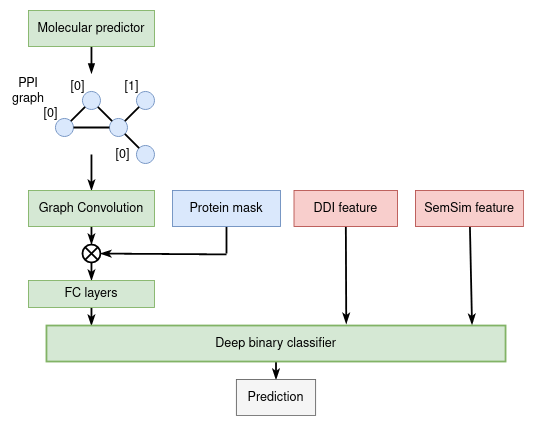
\includegraphics[width=0.4\textwidth]{figures/InteractionNetwork.png}}
\caption{Deep neural network that predicts based on drug-drug interaction features and semantic similarity features over side effects for drugs, and graph convolution over protein-protein interaction networks for proteins. Protein and drug features are represented by blue and red, respectively.}\label{fig:02}
\end{figure}

\section{Discussion}







%%%%%%%%%%%%%%%%%%%%%%%%%%%%%%%%%%%%%%%%%%%%%%%%%%%%%%%%%%%%%%%%%%%%%%%%%%%%%%%%%%%%%
%
%     please remove the " % " symbol from \centerline{\includegraphics{fig01.eps}}
%     as it may ignore the figures.
%
%%%%%%%%%%%%%%%%%%%%%%%%%%%%%%%%%%%%%%%%%%%%%%%%%%%%%%%%%%%%%%%%%%%%%%%%%%%%%%%%%%%%%%






\section{Conclusion}

\vspace*{-10pt}


\section*{Acknowledgements}

\vspace*{-12pt}

\section*{Funding}

This work has been supported by the... Text Text  Text Text.\vspace*{-12pt}

%\bibliographystyle{natbib}
%\bibliographystyle{achemnat}
%\bibliographystyle{plainnat}
%\bibliographystyle{abbrv}
%\bibliographystyle{bioinformatics}
%
%\bibliographystyle{plain}
%
\bibliography{citations}


\end{document}

%%% Local Variables:
%%% mode: latex
%%% TeX-master: t
%%% End:
